
\section{Characterization of critical windows}\label{sec:master}

Let $\Sinit\subset\Theta$ denote some sub-mixture, corresponding to a sub-population of $p$ that possesses a certain property. For instance, if $p$ corresponds to some autoregressive model, $\Sinit$ might correspond to sentences which correctly answer a particular math question. Let $\Send\supset\Sinit$ denote some sub-mixture containing $\Sinit$. For instance, $\Send$ might correspond to all possible responses to the math question, including incorrect ones.

We are interested in the following question: if we run the forward-reverse experiment for time $\wh{T}$ starting from $p^{\Sinit}$, is there some range of times for which the resulting distribution is close to $p^{\Send}$? That is, can we characterize the $\wh{T}$ for which
\begin{equation}
    \TV(\modrevlaw{\Sinit}{\wh{T}}{}, p^{\Send})
\end{equation}
is small?

Suppose one could prove that the range of $\wh{T}$ for which this is the case is some interval $[T_0, T_1]$. This would mean that if the stochastic localization sampler runs for time $T$ and ends up at a sample from $p^{\Sinit}$, then from time $T - T_1$ to time $T - T_0$ of the generation process, \emph{the sampler has not yet localized the features that distinguish $p^{\Sinit}$ from the larger sub-mixture $p^{\Send}$}. However, the sampler has localized the features that distinguish $p^{\Send}$ from $p^{\Theta-\Send}$. When there is a shift from localizing the features $\Send$ to the features $\Sinit$, we say there is a critical window. We now formally state and prove our main result.  

\subsection{Main result} 

For an error parameter $0 < \epsilon < 1$, define
\begin{align*} 
\Tupper(\epsilon) \in \sup\{&t \in \I:\TV(p_{t}^{\Send}  ,p_{t}^{\Theta-\Send }) \geq 1-\epsilon^2\,\} \\
\Tlower(\epsilon) \in  \inf\{&t \in  \I:  \TV(p_{t}^{S_{\mathrm{init}}  },p_{t}^{\Send }) \leq \epsilon\}\,.
\end{align*} 
This is well-defined for continuous observation processes.\footnote{For general stochastic localization schemes, we can only ask that $\Tupper(\epsilon) \in  \{ r\in \I:\TV(p_{t}^{\Send} ,p_{t}^{\Theta-\Send }) \geq 1-\epsilon^2\,\}$ and $\Tlower(\epsilon) \in  \{t \in  \I:  \TV(p_{t}^{S_{\mathrm{init}}  },p_{t}^{\Send }) \leq \epsilon\}$ instead of $\sup,\inf$ like \citep{li2024criticalwindowsnonasymptotictheory}, because the sets $ \{t \in \I:\TV(p_{t}^{\Send}  ,p_{t}^{\Theta-\Send }) \geq 1-\epsilon^2\,\},\{t \in  \I:  \TV(p_{t}^{S_{\mathrm{init}}  },p_{t}^{\Send }) \leq \epsilon\}$ may not be closed for observation processes which are discontinuous. For autoregressive language models and continuous diffusion, the observation process is continuous, so we will elide these technicalities.
.} When the value of $\epsilon$ is understood, we abbreviate the above with $\Tupper$ and $\Tlower$.  Our main result is that in $\wh{T}\in \I \cap [\Tlower,\Tupper]$, the distance $\TV(\modrevlaw{\Sinit}{\wh{T}}{}, p^{\Send})$ is small:

\begin{theorem}\label{thm:masters_theorem} 
Let $S_{\mathrm{init}}\subset \Send \subset \Theta$ and $W=\frac{\sum_{\theta \in \Theta-\Send} w_\theta}{\sum_{\theta \in \Send} w_\theta}$. For $\epsilon > 0$, if $\wh{T}\in \I \cap [\Tlower,\Tupper]$, then  
$\TV(\modrevlaw{\Sinit}{\wh{T}}{}, p^{\Send}) \leq \epsilon\cdot\bigl(1+\max\left(1,W\right)/\sqrt{2}\bigr).$
\end{theorem}
Intuitively, $\Tupper$ represents the largest $t$ for which there is still separation between $\Send$ and $\Theta-\Send$, and $\Tlower$ represents the smallest $t$ for which samples from $\Sinit,\Send$ are indistinguishable. Thus, running it for $\wh{T}\in \I \cap [\Tlower,\Tupper]$ erases the differences between samples from $\Sinit$ and $\Send$ but preserves the difference between $\Send$ and $\Theta-\Send$, yielding samples looking like $p^{\Send}$.
\begin{remark}
\emph{A priori} it is not clear why $\Tlower$ should be smaller than $\Tupper$, and indeed in general it need not be and our bound would be vacuous. In Section~\ref{sec:eg_theory} however, we show that in many natural settings for diffusion models and autoregressive models, the relation does hold.
\end{remark}
\begin{remark}
Note a similar bound was shown in the context of diffusions by \cite{li2024criticalwindowsnonasymptotictheory} (see Theorem 7 therein), who used an approximation argument from~\cite{DBLP:conf/iclr/ChenC0LSZ23} and Girsanov's theorem to prove thei results. Our result is a strict improvement of that bound along several important axes. First, our results apply to all stochastic localization samplers, not just diffusions. This is because our proof is extremely simple and does not require any stochastic calculus. Secondly, \cite{li2024criticalwindowsnonasymptotictheory} needed to assume that the components of $p$ were strongly log-concave and that the score, i.e. gradient of the log-density, of $p_t$ was Lipschitz and moment-bounded for all $t$. Thirdly, their final bound includes a polynomial dependence on the moments of the score, which scale with the dimension $d$; in contrast, our final bound is independent of $d$. 

\end{remark}

With Theorem~\ref{thm:masters_theorem} in place, we are ready to formally define \emph{critical windows}. These capture the moments where we transition from sampling from a sub-mixture to a subset of that sub-mixture.
\begin{definition}
Define $\Safter \subset \Sbefore \subset \Theta$. For $\Sbefore$, we define $\Tbefore =\inf\{t \in \I:\TV(p_t^{\Safter},p_t^{\Sbefore}) \leq \epsilon \text{ and } \TV(p_t^{\Sbefore},p_t^{\Theta-\Sbefore})\geq 1- \epsilon^2\}$ ($\Sinit\triangleq \Safter;\Send\triangleq \Sbefore)$. For $\Safter$, consider $\Tafter = \sup \{t \in \I:\TV(p_t^{\Safter},p_t^{\Theta-\Safter}) \geq 1-\epsilon^2\}$ ($\Sinit,\Send\triangleq\Safter$). A \textbf{critical window} is the interval $[\Tafter,\Tbefore]$, where there is a transition from sampling from $\Sbefore$ to the smaller subset $\Safter$. 
\end{definition}
\begin{figure}[H]
\centering
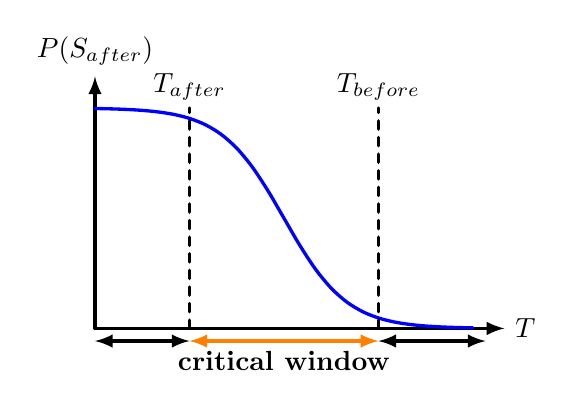
\begin{tikzpicture}[>=latex, line cap=round, scale=0.8,line join=round]
% Axes
\draw[->,very thick] (0,0) -- (6.5,0) node[right] {$T$};
\draw[->,very thick] (0,0) -- (0,4) node[above] {$P(S_{\text{after}})$};

% Probability curve
\draw[very thick,domain=0:6,smooth,variable=\x,color=blue] 
    plot ({\x}, {3.5/(1+exp(2*(\x-3)))});

% Vertical dashed lines
\draw[dashed,very thick] (1.5,0) -- (1.5,3.5);
\draw[dashed,very thick] (4.5,0) -- (4.5,3.5);

% Labels for T_after and T_before
\node[below] at (1.5,4.2) {$T_{\text{after}}$};
\node[below] at (4.5,4.2) {$T_{\text{before}}$};

% Horizontal annotation for critical interval
\draw[<->,very thick] (0,-0.2) -- (1.5,-0.2);
\node[right] at (-0.7,-0.6) {$\Safter$};

\draw[<->,very thick,color=orange] (1.5,-0.2) -- (4.5,-0.2);
\node[below] at (3,-0.2) {\textbf{critical window}};

\draw[<->,very thick] (4.5,-0.2) -- (6.2,-0.2);
\node[right] at (5.2,-0.6) {$\Sbefore$};
\end{tikzpicture}
\caption{Illustration of the definition of a critical window for a simple mixture of two Gaussians, with $\Sbefore\triangleq\{\mathcal{N}(\mu,\mathrm{Id}),\mathcal{N}(-\mu,\mathrm{Id})\}$ and $\Safter\triangleq\{\mathcal{N}(\mu,\mathrm{Id})\}$.}
\label{fig:cw_definition}
\end{figure}
For nonempty $S \subset \Theta$ and $t \in \I$, we define $\kernelreverse[](\cdot |Y_t,S)$ to be the posterior of $X$ with the prior $X \sim p^S$. We similarly define $\kernelreverse[]_{t \to \Theta}(\cdot | Y_t)$ and $\kernelreverse[]_{t \to \Theta}(\cdot | Y_t,S)$ to be the posterior of $\theta$ conditioning on $Y_{t}$ with $X \sim p$ or $X \sim p^S$, respectively. When $S=\{i\}$, we exclude the braces.
\subsection{Proof of Theorem~\ref{thm:masters_theorem}}

\noindent Crucially, our proof relies in several places on the Markov property of stochastic localization samplers, together with the data processing inequality. 

\begin{proof}[Proof of Theorem~\ref{thm:masters_theorem}]
By the triangle inequality, we can write
\begin{align*}
\TV(\modrevlawX{\Sinit}{\wh{T}},p^{\Send})\leq \underbrace{\TV(\modrevlawX{\Sinit}{\wh{T}},\modrevlawX{\Send}{\wh{T}})}_{\text{(I)}}+\underbrace{\TV(\modrevlawX{\Send}{\wh{T}},p^{\Send})}_{\text{(II)}}.
\end{align*}
$\modrevlawX{\Sinit}{\wh{T}}$ and $\modrevlawX{\Send}{\wh{T}}$ are the laws of the posterior $\kernelreverse[](\cdot | \cdot)$ but applied to $Y_{\wh{T}}$ with distributions $p^{\Sinit}_{\wh{T}}$ and $p^{\Send}_{\wh{T}}$. Using the Markov property of localization-based samplers (Definition~\ref{def:observation_process}), we apply the data processing inequality twice and the definition of $\Tlower$ to bound (I) via \[\TV(\modrevlawX{\Sinit}{\wh{T}},\modrevlawX{\Send}{\wh{T}})\leq \TV(p^{S_{\mathrm{init}}  }_{\wh{T}},p^{\Send}_{\wh{T}}) 
 \leq\TV(p^{S_{\mathrm{init}}  }_{\Tlower},p^{\Send}_{\Tlower}) \leq \epsilon.
\]

To bound (II), we use the definition of $\TV$ and a coupling argument. Observe that the observation processes associated with $\modrevlawX{\Send}{\wh{T}}$ and $p^{\Send}$ have the same distribution at index $\wh{T}$. Thus, taking $Y_{\wh{T}} \sim p^{\Send}_{\wh{T}}$, we can express by the law of total probability,
\begin{align*}
\modrevlawX{\Send}{\wh{T}}(x)&=\E[\kernelreverse[](x| Y_{\wh{T}})]\\
p^{\Send}(x)&=\E[\kernelreverse[](x| Y_{\wh{T}},\Send)].
\end{align*}
as these observation processes have the same distribution at index $\wh{T}$. Thus, 
\begin{align*}
\TV(\modrevlawX{\Send}{\wh{T}},p^{\Send}) = \frac{1}{2}  \int \left|\modrevlawX{\Send}{\wh{T}}(x)-p^{\Send}(x) \right|dx=\frac{1}{2} \int \left| \E[\kernelreverse[](x| Y_{\wh{T}})] -\E[\kernelreverse[](x| Y_{\wh{T}},\Send)]. \right|dx.
\end{align*}
By Jensen's inequality and Fubini's theorem, we bring the expectation outside the integral, 
\begin{align*}
\TV(\modrevlawX{\Send}{\wh{T}},p^{\Send}) &\leq \frac{1}{2} \int \E\left[\left|\kernelreverse[](x| Y_{\wh{T}})-\kernelreverse[](x| Y_{\wh{T}},\Send)\right|\right] dx=\frac{1}{2}\E\left[\int \left|\kernelreverse[](x| Y_{\wh{T}})-\kernelreverse[](x| Y_{\wh{T}},\Send)\right| dx\right].
\end{align*}
To simplify the above expression, we use the following two lemmas, proved in App.~\ref{app:master_details}.
\begin{restatable}{lemma}{masterinequality}\label{lem:master_inequality}
By applying the law of total probability and Bayes' rule, we can show for $Y_{\wh{T}}\in\supp(p^{\Send}_{\wh{T}})$,
\begin{align*}
\int \left|\kernelreverse[](x| Y_{\wh{T}})-\kernelreverse[](x| Y_{\wh{T}},\Send)\right| dx \leq  2 \sum_{\theta \in \Theta-\Send} \kernelreverse[]_{t \to \Theta}(\theta|Y_{\wh{T}}).
\end{align*}
\end{restatable} 
\begin{restatable}{lemma}{masterinequalitytwo}\label{lem:master_inequalitytwo}
By Bayes's rule, we can derive for $Y_{\wh{T}} \in \supp(p_{\wh{T}})$,
\begin{align*}
 \sum_{\theta \in \Theta-\Send} \kernelreverse[]_{t \to \Theta}(\theta|Y_{\wh{T}}) \leq  \max\left(1,W\right)  \frac{p^{\Theta-\Send}_{\wh{T}}(Y_{\wh{T}})}{ p^{\Theta-\Send}_{\wh{T}}(Y_{\wh{T}})+p^{\Send}_{\wh{T}}(Y_{\wh{T}})}
\end{align*}
\end{restatable} 
\noindent Combining Lemmas~\ref{lem:master_inequality} and~\ref{lem:master_inequalitytwo} , we find 
\begin{align*}
\TV(\modrevlawX{\Send}{\wh{T}},p^{\Send}) \leq \max\left(1,W\right) \E\left[ \frac{p^{\Theta-\Send}_{\wh{T}}(Y_{\wh{T}})}{ p^{\Theta-\Send}_{\wh{T}}(Y_{\wh{T}})+p^{\Send}_{\wh{T}}(Y_{\wh{T}})}\right]. 
\end{align*}
Then, finally applying Lemma~\ref{lem:ratio_inequality}, we are able to bound the total variation in terms of $\epsilon$, 
\begin{align*}
\TV(\modrevlawX{\Send}{\wh{T}},p^{\Send}) \leq \frac{1}{2}\max\left(1,W\right) \sqrt{1-\TV^2(p^{\Theta-\Send}_{\wh{T}},p^{\Send}_{\wh{T}})}\leq \frac{\sqrt{2}}{2}\max\left(1,W\right) \epsilon.
\end{align*}
\noindent Combining our bounds on (I) and (II) achieves the desired result.
\end{proof}

